\documentclass{standalone}
\usepackage{tikz}
\usetikzlibrary{calc}

\begin{document}
  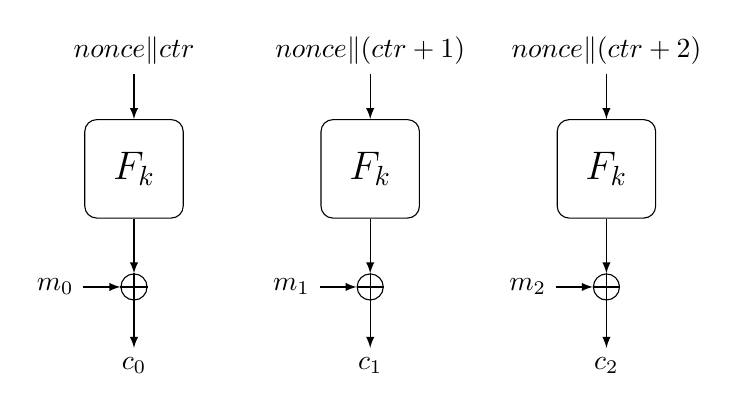
\begin{tikzpicture}
    \foreach \x in {0, 1, 2} {
      \node (f\x) at ($\x*(3.0cm,0)$) [minimum size=1.25cm,rounded corners=1ex,draw] {\Large $F_k$};
      \node (c\x) [below of=f\x, node distance=2.5cm] {$c_\x$};
      % \node (k\x) [left of=f\x, node distance=1.5cm] {$k$};
      \node (p\x) [below of=f\x, node distance=1.5cm, circle, draw] {};
      \node (m\x) [left of=p\x, node distance=1.0cm] {$m_\x$};
      \draw[-] (p\x.north) -- (p\x.south);
      \draw[-] (p\x.east) -- (p\x.west);
      \draw[-latex] (m\x) -- (p\x);
      \draw[-latex] (f\x) -- (p\x);
      \draw[-latex] (p\x) -- (c\x);
    }

    \node (n0) [above of=f0, node distance=1.5cm] {$nonce\|ctr$};
    \node (n1) [above of=f1, node distance=1.5cm] {$nonce\|(ctr+1)$};
    \node (n2) [above of=f2, node distance=1.5cm] {$nonce\|(ctr+2)$};
    \draw[-latex] (n0) -- (f0);
    \draw[-latex] (n1) -- (f1);
    \draw[-latex] (n2) -- (f2);
  \end{tikzpicture}
\end{document}
